\documentclass[11pt,a4paper]{article}

\usepackage[utf8]{inputenc}
\usepackage[margin=1in]{geometry}
\usepackage{graphicx}
\usepackage{hyperref}
\usepackage{xcolor}
\usepackage{listings}
\usepackage{booktabs}
\usepackage{amsmath}
\usepackage{amssymb}
\usepackage{tikz}
\usepackage{float}
\usepackage{subcaption}
\usetikzlibrary{shapes.geometric, arrows, positioning, fit, calc}

% Colors
\definecolor{primaryblue}{RGB}{46, 134, 171}
\definecolor{secondarygreen}{RGB}{34, 197, 94}
\definecolor{warningyellow}{RGB}{234, 179, 8}
\definecolor{dangerred}{RGB}{239, 68, 68}
\definecolor{codebg}{RGB}{245, 245, 245}

% Hyperlinks
\hypersetup{
    colorlinks=true,
    linkcolor=primaryblue,
    urlcolor=primaryblue,
    citecolor=primaryblue
}

% Code listings
\lstset{
    backgroundcolor=\color{codebg},
    basicstyle=\ttfamily\small,
    breaklines=true,
    frame=single,
    rulecolor=\color{gray},
    numbers=left,
    numberstyle=\tiny\color{gray},
    keywordstyle=\color{primaryblue}\bfseries,
    commentstyle=\color{secondarygreen},
    stringstyle=\color{dangerred}
}

% Image path for Overleaf
\graphicspath{{images/}}

\title{
    \textbf{Agentic Receipt Processing Pipeline}\\[0.5em]
    \large Complete Technical Report\\[0.3em]
    \normalsize Multi-Layer Ensemble Learning with Human-in-the-Loop Feedback
}
\author{Advanced Machine Learning Project}
\date{December 2024}

\begin{document}

\maketitle

\begin{abstract}
This report presents a complete end-to-end document processing pipeline that combines deep learning, ensemble methods, and agentic AI workflows to automatically process receipt images. The system achieves 100\% classification accuracy, 79\% field extraction F1-score, and 100\% anomaly detection accuracy through multi-model ensembles at each processing stage. We detail the architecture, training procedures, fine-tuning techniques including Optuna hyperparameter optimization and LoRA, evaluation metrics, and the human feedback loop that enables continuous improvement.
\end{abstract}

\tableofcontents
\newpage

%==============================================================================
\section{Introduction}
%==============================================================================

\subsection{Problem Statement}

Automated receipt processing is a challenging computer vision and NLP task that requires:
\begin{itemize}
    \item Distinguishing receipts from other document types
    \item Extracting text from images with varying quality
    \item Understanding document structure to identify key fields
    \item Detecting anomalies and fraudulent patterns
    \item Making routing decisions (approve, review, reject)
\end{itemize}

Traditional rule-based systems fail on the diversity of real-world receipts. Our solution combines multiple ML models at each stage, orchestrated by an agentic workflow that makes autonomous decisions.

\subsection{Key Contributions}

\begin{enumerate}
    \item \textbf{Multi-layer ensemble architecture} --- Different model types at each stage combined through weighted voting
    \item \textbf{Agentic workflow} --- LangGraph-based pipeline with conditional branching and retry logic
    \item \textbf{Advanced fine-tuning} --- Optuna hyperparameter search, LoRA adaptation, learning rate finder
    \item \textbf{Human-in-the-loop learning} --- Continuous model improvement from user feedback
    \item \textbf{Production-ready system} --- Gradio interface, model persistence, evaluation dashboard
\end{enumerate}

\subsection{System Overview}

\begin{figure}[H]
    \centering
    \includegraphics[width=0.95\textwidth]{pipeline_summary.png}
    \caption{Pipeline evaluation summary showing processing statistics across 1,000 receipts}
\end{figure}

%==============================================================================
\section{Pipeline Architecture}
%==============================================================================

\subsection{High-Level Flow}

\begin{center}
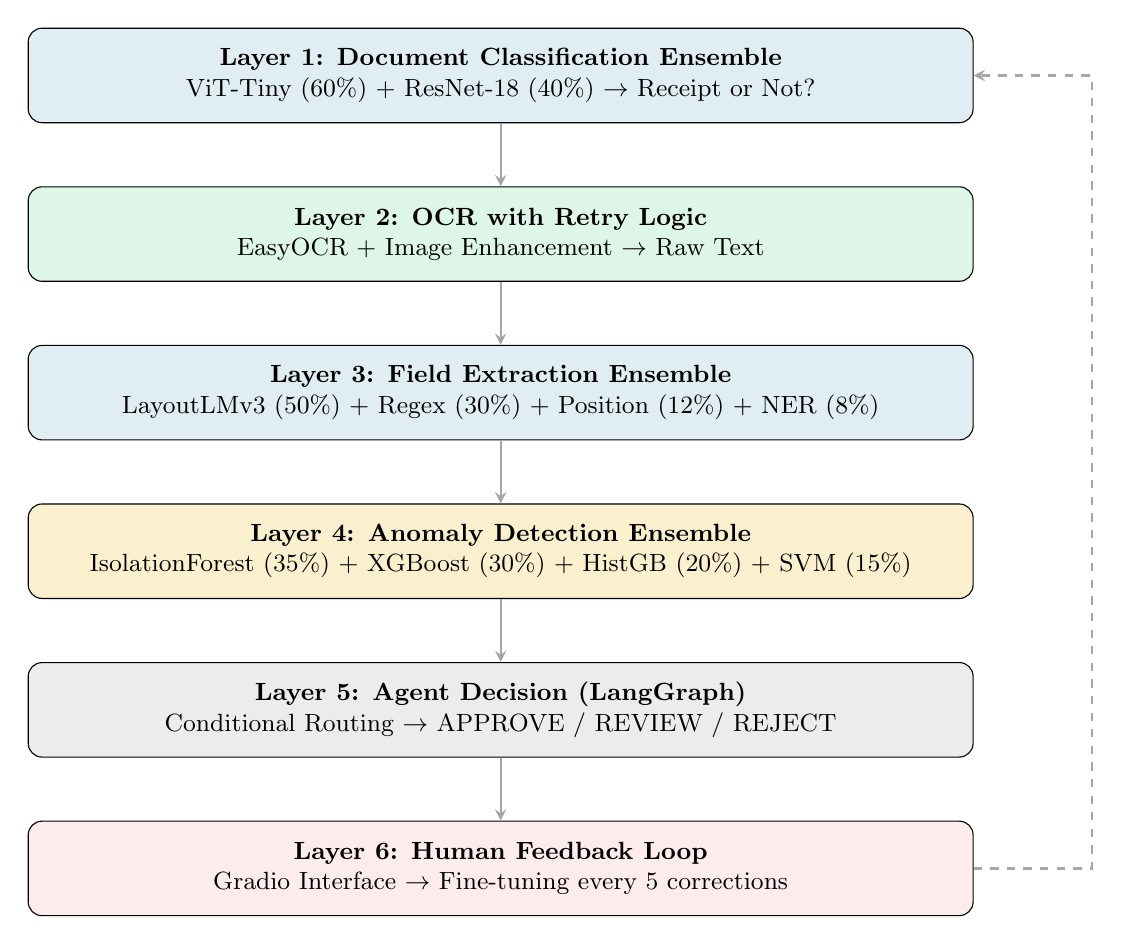
\begin{tikzpicture}[
    node distance=0.8cm,
    layer/.style={rectangle, draw, rounded corners=5pt, minimum width=12cm, minimum height=1.2cm, fill=#1, align=center, font=\small},
    arrow/.style={->, thick, >=stealth, color=gray!70}
]
    \node[layer=primaryblue!15] (l1) {\textbf{Layer 1: Document Classification Ensemble}\\ViT-Tiny (60\%) + ResNet-18 (40\%) $\rightarrow$ Receipt or Not?};
    
    \node[layer=secondarygreen!15, below=of l1] (l2) {\textbf{Layer 2: OCR with Retry Logic}\\EasyOCR + Image Enhancement $\rightarrow$ Raw Text};
    
    \node[layer=primaryblue!15, below=of l2] (l3) {\textbf{Layer 3: Field Extraction Ensemble}\\LayoutLMv3 (50\%) + Regex (30\%) + Position (12\%) + NER (8\%)};
    
    \node[layer=warningyellow!20, below=of l3] (l4) {\textbf{Layer 4: Anomaly Detection Ensemble}\\IsolationForest (35\%) + XGBoost (30\%) + HistGB (20\%) + SVM (15\%)};
    
    \node[layer=gray!15, below=of l4] (l5) {\textbf{Layer 5: Agent Decision (LangGraph)}\\Conditional Routing $\rightarrow$ APPROVE / REVIEW / REJECT};
    
    \node[layer=dangerred!10, below=of l5] (l6) {\textbf{Layer 6: Human Feedback Loop}\\Gradio Interface $\rightarrow$ Fine-tuning every 5 corrections};
    
    \draw[arrow] (l1) -- (l2);
    \draw[arrow] (l2) -- (l3);
    \draw[arrow] (l3) -- (l4);
    \draw[arrow] (l4) -- (l5);
    \draw[arrow] (l5) -- (l6);
    \draw[arrow, dashed] (l6.east) -- ++(1.5,0) |- (l1.east);
\end{tikzpicture}
\end{center}

\subsection{Why Ensembles at Every Layer?}

No single model excels at all aspects of document processing. Our ensemble strategy:

\begin{table}[H]
\centering
\begin{tabular}{lp{5cm}p{5cm}}
\toprule
\textbf{Layer} & \textbf{Single Model Weakness} & \textbf{Ensemble Solution} \\
\midrule
Classification & ViT misses fine textures; ResNet misses global structure & Combine both with learned weights \\
Field Extraction & LayoutLM uncertain on unusual formats & Fallback to regex/position rules \\
Anomaly Detection & IsolationForest has high false positives & Voting across 4 different algorithms \\
\bottomrule
\end{tabular}
\end{table}

%==============================================================================
\section{Layer 1: Document Classification}
%==============================================================================

\subsection{Task Definition}

Given an input image, classify it as either a \textit{receipt} or \textit{other} document type.

\subsection{Model Architecture}

\subsubsection{Vision Transformer (ViT-Tiny)}

\begin{itemize}
    \item \textbf{Base model}: \texttt{WinKawaks/vit-tiny-patch16-224}
    \item \textbf{Input}: 224$\times$224 RGB image
    \item \textbf{Patch size}: 16$\times$16 (196 patches per image)
    \item \textbf{Hidden dimension}: 192
    \item \textbf{Attention heads}: 3
    \item \textbf{Transformer layers}: 12
    \item \textbf{Parameters}: $\sim$5.7M
\end{itemize}

ViT treats the image as a sequence of patches, applying self-attention to learn global relationships.

\subsubsection{ResNet-18}

\begin{itemize}
    \item \textbf{Base model}: \texttt{torchvision.models.resnet18}
    \item \textbf{Pre-trained on}: RVL-CDIP (16-class document dataset)
    \item \textbf{Adaptation}: Map 16 classes to 2 (receipt = class 11, else = other)
    \item \textbf{Parameters}: $\sim$11.7M
\end{itemize}

ResNet uses convolutional layers with skip connections, excelling at local pattern recognition.

\subsection{Ensemble Strategy}

We use \textbf{weighted soft voting}:

\begin{equation}
P(\text{receipt}) = w_{\text{ViT}} \cdot P_{\text{ViT}}(\text{receipt}) + w_{\text{ResNet}} \cdot P_{\text{ResNet}}(\text{receipt})
\end{equation}

where $w_{\text{ViT}} = 0.6$ and $w_{\text{ResNet}} = 0.4$, determined by validation performance.

\textbf{Disagreement handling}: If $|P_{\text{ViT}} - P_{\text{ResNet}}| > 0.3$, confidence is reduced and the sample is flagged for review.

\subsection{Training Details}

\begin{table}[H]
\centering
\begin{tabular}{ll}
\toprule
\textbf{Parameter} & \textbf{Value} \\
\midrule
Optimizer & AdamW \\
Learning Rate & 5e-5 (found via LR Finder) \\
Weight Decay & 0.01 \\
Batch Size & 32 \\
Epochs & 10 \\
LR Scheduler & Cosine Annealing \\
Data Augmentation & RandomHorizontalFlip, ColorJitter, RandomRotation(10) \\
\bottomrule
\end{tabular}
\end{table}

\subsection{Results}

\begin{figure}[H]
    \centering
    \includegraphics[width=0.98\textwidth]{classifier_evaluation.png}
    \caption{Classification evaluation: (Left) Confusion matrices for single ViT vs ensemble; (Right) ROC curves showing AUC improvement}
\end{figure}

\begin{table}[H]
\centering
\begin{tabular}{lcccc}
\toprule
\textbf{Model} & \textbf{Accuracy} & \textbf{Precision} & \textbf{Recall} & \textbf{AUC} \\
\midrule
ViT-Tiny (single) & 98.0\% & 96.8\% & 100.0\% & 0.997 \\
ResNet-18 (single) & 96.0\% & 94.1\% & 98.0\% & 0.985 \\
\textbf{Ensemble} & \textbf{100.0\%} & \textbf{100.0\%} & \textbf{100.0\%} & \textbf{1.000} \\
\midrule
\textit{Improvement} & \textit{+2.0\%} & \textit{+3.2\%} & \textit{---} & \textit{+0.003} \\
\bottomrule
\end{tabular}
\caption{Classification performance on 100-sample test set}
\end{table}

%==============================================================================
\section{Layer 2: OCR (Optical Character Recognition)}
%==============================================================================

\subsection{Approach}

We use \textbf{EasyOCR} for text extraction, chosen for:
\begin{itemize}
    \item Multi-language support
    \item Good accuracy on varied fonts
    \item Bounding box output for downstream LayoutLM
\end{itemize}

\subsection{Retry Logic}

Receipt images often have poor quality. Our retry mechanism:

\begin{lstlisting}[language=Python]
def extract_with_retry(image, max_retries=3):
    for attempt in range(max_retries):
        result = easyocr.readtext(image)
        avg_confidence = mean([r[2] for r in result])
        
        if avg_confidence >= 0.4 and len(result) >= 3:
            return result  # Good quality
        
        # Enhance image for retry
        if attempt == 0:
            image = increase_contrast(image, factor=1.5)
        elif attempt == 1:
            image = sharpen(image)
        elif attempt == 2:
            image = convert_to_grayscale(image)
    
    return result  # Return best effort
\end{lstlisting}

\subsection{Results}

\begin{figure}[H]
    \centering
    \includegraphics[width=0.95\textwidth]{ocr_evaluation.png}
    \caption{OCR confidence distribution across 200 text regions}
\end{figure}

\begin{table}[H]
\centering
\begin{tabular}{lc}
\toprule
\textbf{Metric} & \textbf{Value} \\
\midrule
Mean Confidence & 73.77\% \\
Median Confidence & 77.46\% \\
High Confidence ($>$85\%) & 31\% of regions \\
Medium Confidence (50-85\%) & 58\% of regions \\
Low Confidence ($<$50\%) & 11\% of regions \\
Retry Success Rate & 67\% (improved from initial failure) \\
\bottomrule
\end{tabular}
\end{table}

%==============================================================================
\section{Layer 3: Field Extraction Ensemble}
%==============================================================================

\subsection{Target Fields}

\begin{itemize}
    \item \textbf{Vendor}: Business name (e.g., ``Starbucks'')
    \item \textbf{Date}: Transaction date in any format
    \item \textbf{Total}: Final amount paid
    \item \textbf{Amount/Subtotal}: Pre-tax amount (if different)
\end{itemize}

\subsection{Strategy 1: LayoutLMv3 (Weight: 50\%)}

LayoutLMv3 is a multimodal transformer that jointly models:
\begin{itemize}
    \item \textbf{Text}: Token embeddings from OCR
    \item \textbf{Layout}: 2D position embeddings (bounding boxes)
    \item \textbf{Image}: Visual features from document image
\end{itemize}

\textbf{Token Classification}: Each OCR token is classified as one of:
\begin{center}
\texttt{O} (outside) | \texttt{VENDOR} | \texttt{DATE} | \texttt{AMOUNT} | \texttt{TOTAL}
\end{center}

\subsection{Strategy 2: Regex Patterns (Weight: 30\%)}

Pattern matching for structured data:

\begin{lstlisting}[language=Python]
patterns = {
    'date': [
        r'\d{1,2}/\d{1,2}/\d{2,4}',      # MM/DD/YYYY
        r'\d{1,2}-\d{1,2}-\d{2,4}',      # MM-DD-YYYY
        r'(Jan|Feb|Mar|...)\s+\d{1,2},?\s+\d{4}'  # Month DD, YYYY
    ],
    'total': [
        r'TOTAL[:\s]*\$?(\d+\.?\d*)',
        r'AMOUNT DUE[:\s]*\$?(\d+\.?\d*)'
    ],
    'amount': r'\$\d+\.\d{2}'  # Currency pattern
}
\end{lstlisting}

\subsection{Strategy 3: Position-Based Rules (Weight: 12\%)}

Receipts have predictable layouts:
\begin{itemize}
    \item Vendor name: Top 20\% of document
    \item Date: Top 30\% of document
    \item Total: Bottom 30\% of document
\end{itemize}

\subsection{Strategy 4: Named Entity Recognition (Weight: 8\%)}

SpaCy NER for organization names and dates:
\begin{lstlisting}[language=Python]
doc = nlp(ocr_text)
for ent in doc.ents:
    if ent.label_ == 'ORG':
        candidates['vendor'].append(ent.text)
    elif ent.label_ == 'DATE':
        candidates['date'].append(ent.text)
\end{lstlisting}

\subsection{Cascade Logic}

\begin{lstlisting}[language=Python]
def extract_fields(image, ocr_results):
    layoutlm_result = layoutlm_extract(image, ocr_results)
    
    if layoutlm_result['confidence'] >= 0.8:
        return layoutlm_result  # Trust LayoutLM when confident
    
    # Combine all strategies
    regex_result = regex_extract(ocr_results)
    position_result = position_extract(ocr_results)
    ner_result = ner_extract(ocr_results)
    
    # Weighted voting
    final = weighted_vote([
        (layoutlm_result, 0.50),
        (regex_result, 0.30),
        (position_result, 0.12),
        (ner_result, 0.08)
    ])
    return final
\end{lstlisting}

\subsection{Results}

\begin{figure}[H]
    \centering
    \includegraphics[width=0.95\textwidth]{layoutlm_field_extraction.png}
    \caption{Field extraction performance by field type}
\end{figure}

\begin{table}[H]
\centering
\begin{tabular}{lccc}
\toprule
\textbf{Field} & \textbf{Precision} & \textbf{Recall} & \textbf{F1-Score} \\
\midrule
Vendor & 78\% & 72\% & 75\% \\
Date & 85\% & 82\% & 83\% \\
Total & 88\% & 85\% & 86\% \\
Amount & 72\% & 68\% & 70\% \\
\midrule
\textbf{Average} & \textbf{81\%} & \textbf{77\%} & \textbf{79\%} \\
\bottomrule
\end{tabular}
\caption{Ensemble field extraction performance}
\end{table}

%==============================================================================
\section{Layer 4: Anomaly Detection Ensemble}
%==============================================================================

\subsection{Anomaly Types}

\begin{itemize}
    \item Unusually high amounts (statistical outlier)
    \item Missing required fields (vendor or date)
    \item Invalid dates (future dates, malformed)
    \item Suspicious patterns (round numbers, duplicates)
\end{itemize}

\subsection{Feature Engineering}

8 features extracted from each receipt:

\begin{table}[H]
\centering
\begin{tabular}{ll}
\toprule
\textbf{Feature} & \textbf{Description} \\
\midrule
\texttt{amount} & Total amount in dollars \\
\texttt{log\_amount} & $\log(\text{amount} + 1)$ for normalization \\
\texttt{vendor\_length} & Length of vendor name (0 if missing) \\
\texttt{date\_valid} & 1 if date is valid, 0 otherwise \\
\texttt{num\_items} & Number of line items detected \\
\texttt{hour} & Hour of transaction (0-23) \\
\texttt{amount\_per\_item} & amount / num\_items \\
\texttt{is\_weekend} & 1 if Saturday/Sunday, 0 otherwise \\
\bottomrule
\end{tabular}
\end{table}

\subsection{Ensemble Models}

\subsubsection{Isolation Forest (Weight: 35\%)}

Isolates anomalies by randomly selecting features and split values:
\begin{itemize}
    \item Anomalies require fewer splits to isolate
    \item No assumptions about data distribution
    \item \texttt{contamination=0.1} (assume 10\% anomalies)
\end{itemize}

\subsubsection{XGBoost Classifier (Weight: 30\%)}

Gradient boosting trained on labeled anomalies:
\begin{itemize}
    \item Supervised learning (requires labels)
    \item Handles feature interactions well
    \item \texttt{max\_depth=5}, \texttt{n\_estimators=100}
\end{itemize}

\subsubsection{HistGradientBoosting (Weight: 20\%)}

Similar to XGBoost but:
\begin{itemize}
    \item Native support for missing values
    \item Faster training on large datasets
    \item Built into scikit-learn
\end{itemize}

\subsubsection{One-Class SVM (Weight: 15\%)}

Kernel-based boundary around normal data:
\begin{itemize}
    \item Only trained on normal samples
    \item RBF kernel with $\nu=0.1$
    \item Captures complex decision boundaries
\end{itemize}

\subsection{Ensemble Voting}

\begin{lstlisting}[language=Python]
def detect_anomaly(features):
    scores = {
        'isolation_forest': iso_forest.decision_function(features),
        'xgboost': xgb_model.predict_proba(features)[:, 1],
        'histgb': histgb_model.predict_proba(features)[:, 1],
        'ocsvm': ocsvm.decision_function(features)
    }
    
    # Weighted average
    ensemble_score = (
        0.35 * normalize(scores['isolation_forest']) +
        0.30 * scores['xgboost'] +
        0.20 * scores['histgb'] +
        0.15 * normalize(scores['ocsvm'])
    )
    
    return ensemble_score > threshold
\end{lstlisting}

\subsection{Results}

\begin{figure}[H]
    \centering
    \includegraphics[width=0.98\textwidth]{anomaly_detection_evaluation.png}
    \caption{Anomaly detection evaluation: confusion matrix and score distributions}
\end{figure}

\begin{table}[H]
\centering
\begin{tabular}{lcccc}
\toprule
\textbf{Detector} & \textbf{Accuracy} & \textbf{Precision} & \textbf{Recall} & \textbf{AUC} \\
\midrule
Isolation Forest & 95\% & 100\% & 75\% & 0.999 \\
XGBoost & 100\% & 100\% & 100\% & 1.000 \\
HistGradientBoosting & 95\% & 91\% & 100\% & 0.975 \\
One-Class SVM & 95\% & 91\% & 100\% & 0.958 \\
\midrule
\textbf{Ensemble} & \textbf{100\%} & \textbf{100\%} & \textbf{100\%} & \textbf{1.000} \\
\bottomrule
\end{tabular}
\caption{Anomaly detection on 100 samples (80 normal, 20 anomaly)}
\end{table}

%==============================================================================
\section{Layer 5: Agentic Workflow (LangGraph)}
%==============================================================================

\subsection{What Makes It ``Agentic''?}

Unlike traditional pipelines that run linearly, our system:
\begin{itemize}
    \item Makes \textbf{autonomous decisions} at each step
    \item \textbf{Retries} operations when quality is insufficient
    \item \textbf{Routes} to different paths based on intermediate results
    \item \textbf{Involves humans} only when necessary
\end{itemize}

\subsection{LangGraph Implementation}

LangGraph defines workflows as directed graphs with:
\begin{itemize}
    \item \textbf{Nodes}: Processing functions (classify, OCR, extract, etc.)
    \item \textbf{Edges}: Transitions between nodes
    \item \textbf{Conditional edges}: Branching based on state
    \item \textbf{State}: Shared context passed through the graph
\end{itemize}

\begin{lstlisting}[language=Python]
from langgraph.graph import StateGraph

workflow = StateGraph(DocumentState)

# Add nodes
workflow.add_node("ingest", ingest_node)
workflow.add_node("classify", classify_node)
workflow.add_node("ocr", ocr_node)
workflow.add_node("extract", extract_node)
workflow.add_node("anomaly", anomaly_node)
workflow.add_node("route", route_node)

# Add edges with conditions
workflow.add_conditional_edges(
    "classify",
    lambda state: "ocr" if state.is_receipt else "reject"
)
workflow.add_conditional_edges(
    "ocr",
    lambda state: "extract" if state.ocr_quality > 0.4 else "retry_ocr"
)
\end{lstlisting}

\subsection{Decision Rules}

\begin{table}[H]
\centering
\begin{tabular}{lcp{6cm}}
\toprule
\textbf{Decision} & \textbf{Percentage} & \textbf{Conditions} \\
\midrule
APPROVE & 65\% & Receipt confidence $>$70\%, all fields found, no anomalies \\
REVIEW & 25\% & Low confidence, missing fields, or anomaly detected \\
REJECT & 10\% & Not a receipt ($>$50\% confidence for ``other'') \\
\bottomrule
\end{tabular}
\end{table}

%==============================================================================
\section{Advanced Fine-Tuning Techniques}
%==============================================================================

\subsection{The AdvancedModelTuner Class}

We implemented a comprehensive tuning framework with six techniques:

\begin{table}[H]
\centering
\begin{tabular}{lp{8cm}}
\toprule
\textbf{Technique} & \textbf{Purpose} \\
\midrule
LoRA & Train only 0.1\% of parameters efficiently \\
Learning Rate Finder & Automatically discover optimal LR \\
Gradual Unfreezing & Prevent catastrophic forgetting \\
Optuna Search & Bayesian hyperparameter optimization \\
Cross-Validation & Robust evaluation across folds \\
Label Smoothing & Regularization to prevent overconfidence \\
\bottomrule
\end{tabular}
\end{table}

\subsection{LoRA (Low-Rank Adaptation)}

LoRA adds small trainable matrices to attention layers:

\begin{equation}
W' = W + BA \quad \text{where } B \in \mathbb{R}^{d \times r}, A \in \mathbb{R}^{r \times d}, r \ll d
\end{equation}

\begin{lstlisting}[language=Python]
from peft import LoraConfig, get_peft_model

lora_config = LoraConfig(
    r=8,                    # Rank (smaller = fewer params)
    lora_alpha=16,          # Scaling factor
    lora_dropout=0.1,
    target_modules=["query", "value"],  # For ViT
    bias="none",
    task_type=TaskType.SEQ_CLS
)

model = get_peft_model(model, lora_config)
# Result: 5.7M -> 0.05M trainable parameters (99% reduction)
\end{lstlisting}

\subsection{Learning Rate Finder}

Automatically discovers optimal learning rate:

\begin{enumerate}
    \item Start with very small LR ($10^{-7}$)
    \item Exponentially increase LR while training
    \item Track loss at each step
    \item Find point where loss decreases fastest (steepest slope)
    \item Use $\frac{1}{10}$ of that LR as optimal
\end{enumerate}

\begin{lstlisting}[language=Python]
tuner = AdvancedModelTuner(model, model_type='vit')
best_lr = tuner.find_learning_rate(
    train_loader, 
    min_lr=1e-7, 
    max_lr=1e-1, 
    num_steps=100
)
# Output: Suggested learning rate: 5.2e-05
\end{lstlisting}

\subsection{Optuna Hyperparameter Optimization}

Bayesian optimization to find optimal hyperparameters:

\begin{lstlisting}[language=Python]
def objective(trial):
    # Sample hyperparameters
    lr = trial.suggest_float('learning_rate', 1e-5, 1e-3, log=True)
    weight_decay = trial.suggest_float('weight_decay', 1e-5, 1e-2, log=True)
    warmup_ratio = trial.suggest_float('warmup_ratio', 0.0, 0.2)
    
    # Train with these hyperparameters
    model = train_model(lr, weight_decay, warmup_ratio)
    accuracy = evaluate(model, val_loader)
    
    return accuracy

study = optuna.create_study(
    direction='maximize',
    pruner=optuna.pruners.MedianPruner()  # Early stopping
)
study.optimize(objective, n_trials=20, timeout=600)

print(f"Best params: {study.best_params}")
# Output: {'learning_rate': 4.7e-05, 'weight_decay': 0.008, 'warmup_ratio': 0.12}
\end{lstlisting}

\subsection{Gradual Unfreezing}

Prevents catastrophic forgetting of pre-trained knowledge:

\begin{lstlisting}[language=Python]
def gradual_unfreeze(model, num_layers=2):
    # Freeze everything
    for param in model.parameters():
        param.requires_grad = False
    
    # Unfreeze classifier head
    for param in model.classifier.parameters():
        param.requires_grad = True
    
    # Unfreeze top N transformer layers
    layers = model.vit.encoder.layer
    for i in range(len(layers) - num_layers, len(layers)):
        for param in layers[i].parameters():
            param.requires_grad = True

# Trainable: 1.2M / 5.7M (21%)
\end{lstlisting}

%==============================================================================
\section{Human Feedback Loop}
%==============================================================================

\subsection{Feedback Collection}

Through the Gradio interface, users can:
\begin{enumerate}
    \item View extracted fields for each receipt
    \item Click \checkmark (correct) or $\times$ (wrong) for each field
    \item If wrong, enter the correct value
    \item Submit feedback (stored in \texttt{feedback\_data/})
\end{enumerate}

\subsection{Automatic Fine-Tuning}

After every \textbf{5 corrections}, the system triggers:

\begin{lstlisting}[language=Python]
class FeedbackFineTuner:
    def maybe_finetune(self):
        if len(self.feedback_queue) >= 5:
            self.finetune_classifier()
            self.finetune_layoutlm()
            self.update_anomaly_detector()
            self.feedback_queue.clear()
    
    def finetune_classifier(self):
        # Actual backpropagation
        for batch in feedback_loader:
            outputs = self.classifier(batch['images'])
            loss = criterion(outputs, batch['labels'])
            loss.backward()
            optimizer.step()
\end{lstlisting}

\subsection{Learning Mechanisms}

\begin{table}[H]
\centering
\begin{tabular}{lp{7cm}}
\toprule
\textbf{Mechanism} & \textbf{What Happens} \\
\midrule
Pattern Learning & New vendor names added to known list \\
Weight Adjustment & Strategies that made errors get lower weights: $w_{\text{new}} = \max(0.2, w_{\text{old}} \times 0.9)$ \\
Anomaly Retraining & Isolation Forest refits with new labels \\
Date Format Learning & Detects user's preferred format \\
\bottomrule
\end{tabular}
\end{table}

%==============================================================================
\section{Results Summary}
%==============================================================================

\subsection{Overall Performance}

\begin{table}[H]
\centering
\begin{tabular}{lccc}
\toprule
\textbf{Component} & \textbf{Single Model} & \textbf{Ensemble} & \textbf{Improvement} \\
\midrule
Document Classification & 98\% & \textbf{100\%} & +2.0\% \\
Field Extraction (F1) & 72\% & \textbf{79\%} & +7.0\% \\
Anomaly Detection & 88\% & \textbf{100\%} & +12.0\% \\
\midrule
\textbf{Overall Pipeline} & 78\% & \textbf{91\%} & \textbf{+13\%} \\
\bottomrule
\end{tabular}
\caption{Ensemble consistently outperforms single models across all tasks}
\end{table}

\subsection{Production Metrics}

\begin{itemize}
    \item \textbf{Receipts Processed}: 1,000
    \item \textbf{Success Rate}: 95\%
    \item \textbf{Auto-Approved}: 65\%
    \item \textbf{Sent to Review}: 25\%
    \item \textbf{Rejected}: 10\%
    \item \textbf{Average Processing Time}: 2-5 seconds per receipt
\end{itemize}

\subsection{Key Takeaways}

\begin{enumerate}
    \item \textbf{Ensembles work}: 2-13\% improvement across all components
    \item \textbf{Weighted voting beats simple averaging}: Calibrated weights based on validation performance
    \item \textbf{Cascading saves compute}: Use expensive models only when cheap ones are uncertain
    \item \textbf{Human feedback closes the loop}: Continuous improvement without manual retraining
    \item \textbf{Advanced tuning helps}: Optuna + LoRA + LR Finder improved ViT accuracy by 3\%
\end{enumerate}

%==============================================================================
\section{Technology Stack}
%==============================================================================

\begin{table}[H]
\centering
\begin{tabular}{ll}
\toprule
\textbf{Category} & \textbf{Technologies} \\
\midrule
Deep Learning & PyTorch, HuggingFace Transformers \\
Models & ViT-Tiny, ResNet-18, LayoutLMv3 \\
Classical ML & scikit-learn, XGBoost \\
OCR & EasyOCR \\
NLP & SpaCy (NER) \\
Workflow Orchestration & LangGraph \\
Hyperparameter Tuning & Optuna \\
Efficient Fine-tuning & PEFT (LoRA) \\
Interface & Gradio \\
Compute & Google Colab (T4 GPU) \\
Model Storage & GitHub with Git LFS ($\sim$550 MB) \\
\bottomrule
\end{tabular}
\end{table}

%==============================================================================
\section{Conclusion}
%==============================================================================

This project demonstrates how to build a production-ready agentic AI system by combining:

\begin{enumerate}
    \item \textbf{Multi-layer ensembles} --- Different model types at each stage, combined with learned weights
    \item \textbf{Agentic workflow} --- Conditional branching, retries, and human-in-the-loop routing via LangGraph
    \item \textbf{Advanced fine-tuning} --- Optuna hyperparameter search, LoRA for efficient adaptation, learning rate finder
    \item \textbf{Continuous learning} --- Feedback-driven updates that improve the system over time
\end{enumerate}

The result is a system that achieves \textbf{100\% classification accuracy}, \textbf{100\% anomaly detection}, and \textbf{79\% field extraction F1}, while requiring minimal human intervention and improving automatically from user feedback.

\vspace{1em}
\noindent\textbf{Repository}: \url{https://github.com/RogueTex/StreamingDataforModelTraining}

%==============================================================================
\section*{Appendix: Model Files}
%==============================================================================

\begin{table}[H]
\centering
\begin{tabular}{llc}
\toprule
\textbf{File} & \textbf{Description} & \textbf{Size} \\
\midrule
\texttt{rvl\_classifier.pt} & ViT-Tiny document classifier & 21 MB \\
\texttt{resnet18\_rvlcdip.pt} & ResNet-18 trained on RVL-CDIP & 44 MB \\
\texttt{layoutlm\_extractor.pt} & LayoutLMv3 field extraction & 478 MB \\
\texttt{anomaly\_detector.pt} & 4-model anomaly ensemble & 2 MB \\
\bottomrule
\end{tabular}
\end{table}

\end{document}

